\documentclass[a4paper,UTF8]{ctexart}

\usepackage{amsmath, amsthm, amssymb, amsfonts, hyperref, mathrsfs}%美国数学学会的包+?
\usepackage{geometry} %控制界面
\usepackage{bookmark}
\usepackage{fancyhdr} % header & footer
\usepackage{appendix} % 附录
\usepackage{tikz} %作图
\usepackage{graphicx} %插入图片的宏包
\usepackage{float} %设置图片浮动位置的宏包
%\usepackage{subfigure} %插入多图时用子图显示的宏包
\usepackage{listings} %引用代码
\usepackage{physics,mathtools} %物理数学工具
\usepackage{comment}
\usepackage{framed}
\usepackage{caption}
\usepackage{subcaption}
\geometry{top=2.5cm,bottom=2.5cm,left=2.5cm,right=2.5cm} % 布局要求
\pagestyle{fancy} % fancy分格
\fancyhf{} % 清除所有页眉页脚
\renewcommand\headrulewidth{0.6pt}
\renewcommand\footrulewidth{0.6pt}
% font
\setCJKmainfont{Noto Serif CJK SC}[BoldFont={Noto Serif CJK SC Bold}, ItalicFont=]
\lhead{何金铭 PB21020660$\mid$座位号:3}
\cfoot{光的力学效应及光阱PN力的测量实验报告}
\rhead{\thepage}
\lfoot{2024.4.15}
\rfoot{USTC}
%\bibliographystyle{plain} % 引用样式
\everymath{\displaystyle} % display
%============================================================

\begin{document}

\begin{center}
    \textbf{\Large 光的力学效应及光阱PN力的测量实验报告}
    \par \text{\large 何金铭 PB21020660}
\end{center}

\section{实验目的}

光具有能量和动量,光的动量是光的基本属性。携带动量的光与物质相互作用,它们间会有动量的交换,从而表现为光对物体施加一力,作用在物体上的力就等于光引起的单位时间内物体动量的改变。并由此可引起的物体的位移,速度状况的变化,我们称之为光的力学效应。


\section{实验原理}

\subsection{光镊——单光束梯度力光阱}

光作用于物体时,将施加一个力到物体上。由于光辐射对物体产生的力常常表现为压力,因而通常称之为辐射压力或简称光压。然而,在特定的光场分布下,光对物体也可产生一拉力。从而有可能某种特定光场来形成束缚粒子的势阱。

设小球的大小明显大于光波长,可以采用几何光学近似。设小球的折射率$n_1$大于周围媒质的折射率$n_2$。

\begin{figure}[H]
    \centering
    \begin{minipage}[b]{0.9\textwidth}
        \centering
        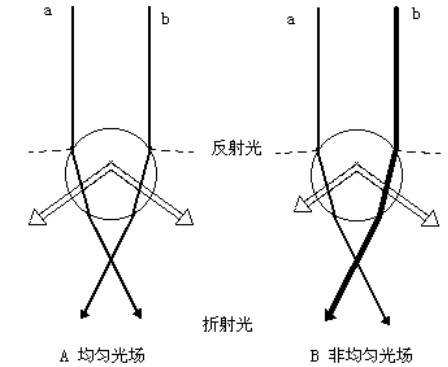
\includegraphics[width=0.6\textwidth]{./fig1.jpg}
        \caption{均匀光场与非均匀光场中的透明小球}
    \end{minipage}
\end{figure}

如果小球处在一个非均匀光场中,如上图B,沿Z方向传播,自左向右光强增大的光场。与左边的光线a相比,
右边较强的光线b作用于小球,使小球获得较大的动量,从而产生较大的力$F_b$。结果总的合力在横向不再平衡,
而是把小球推向右边光强处。小球在这样一个非均匀(即强度分布存在梯度)的光场中所得到的指向光强强的地方的力称之为梯度力($F_g$)

所谓光镊,即单光束梯度力光阱,就是由一束强会聚的激光束构成的。在这样的光场中,粒子
(其折射率$n_1$大于周围煤质的折射率$n_2$)将受到一指向光最强点(焦点)的梯度力。
也就是说光对粒子不仅有推力还可以有拉力。这样,粒子就可能被约束在光最亮点附近。

下图显示了高度会聚的光束锥,经小球折射,将施加一梯度力在小球上。设小球的折射率为n,
液体的折射率为$n_1$,当$n>n_1$时,一对典型的光线a和b经折射后产生力$F_a$和$F_b$,
它们的矢量和是指向焦点f的。实际上,光锥中所有光线施加在小球上的合力F也是指向焦点f的。
当小球的球心O和焦点f间有偏离时,合力F总是使小球趋向焦点。实际上,当光穿过小球时,
在小球表面也产生一定的反射,这将施加一推力于小球,此力常称之为散射力($F_s$)。
只有焦点附近的梯度力大于散射力时才能形成一个三维光学势阱而稳定地捕获微粒。
也就是说,这样的光束可以像镊子一样夹持微粒,移动并操控微粒。

\begin{figure}[H]
    \centering
    \begin{minipage}[b]{0.9\textwidth}
        \centering
        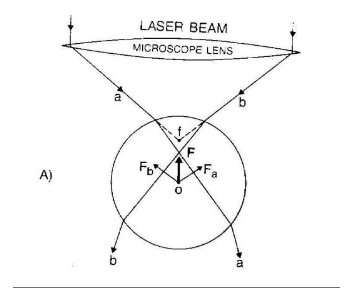
\includegraphics[width=0.6\textwidth]{./fig2.jpg}
        \caption{单光束梯度力光阱原理}
    \end{minipage}
\end{figure}

综上所述,透明微粒在光场中受到的力包括梯度力和散射力($F = F_g + F_s$)。
光阱主要是依靠光梯度力形成的。稳定的捕获是梯度力和散射力平衡的结果。
散射力总是沿光线方向推跑微粒,而梯度力则是把微粒拉向激光的聚焦点处。

\subsection{光阱力测量的流体力学法}

光镊可以捕获和操控微粒,也可以测量作用在微粒上的力。光镊形成的势阱(光阱) 的力学参数在实际应用中十分重要。特别是它的最大捕获力或最大阱力。

光阱力的测量方法大体上有二类:热运动位移法和流体力学法。由于流体力学法具有简单直观的优点,本实验采用了流体力学法。其基本原理如下:

光阱操纵微粒相对流体运动时,微粒将受到液体的粘滞阻力$f$。随着相对速度的增大, 粘滞阻力 $f$ 也随之增大。
当速度超过一定的临界值,粘滞阻力 $f$ 将大于光阱的最大束缚力$F$, 粒子就要从这光阱中逃逸出来。
所以最大阱力${F}_\mathrm{max}$的测量是基于找出光阱操纵微粒所能达到的最大速度 $V_{max}$,
即所谓的逃逸速度。光阱最大阱力 ${F}_\mathrm{max}$的大小就等于这一速度下的粘滞阻力
 $f_{max}$, 但方向相反。在这一速度下的粘滞阻力 $f_{max}$, 可由流体力学中的 Stokes 公式计算:

\begin{equation}
    f_{max}=6\pi \eta r V_{max}
\end{equation}

其中$\eta$为粘滞系数,r 为微粒的半径,$V_{max}$为逃逸速度。

\section{实验结果分析}

1 pixel = 60 nm, 实验室温为$23.0^{\circ}C$, 近似得液体的粘滞系数为:

\begin{equation}
    \eta = 1.005\times 10^{-3} + (0.894-1.005)\times 10^{-3}\cdot \frac{3}{5}  = 0.938 \times 10^{-3} N/m^2\cdot s
\end{equation}

\begin{table}[H]
    \centering
    \caption{测阱域数据记录}
    \begin{tabular}{|l|l|l|l|l|}
    \hline
        $x_1$(pixel) & $y_1$(pixel) & $x_2$(pixel) & $y_2$(pixel) & R(pixel) \\ \hline
        380 & 314 & 426 & 379 & 79.6 \\ \hline
        452 & 321 & 432 & 383 & 65.1 \\ \hline
        289 & 366 & 429 & 384 & 141.2 \\ \hline
    \end{tabular}
\end{table}

得:$\bar{R} = 95.3 \ pixel = 5718 nm = 5.718 \mu m $

\begin{table}[H]
    \centering
    \caption{微粒半径数据记录}
    \begin{tabular}{|l|l|l|l|l|}
    \hline
        $x_1$(pixel) & $y_1$(pixel) & $x_2$(pixel) & $y_2$(pixel) & R(pixel) \\ \hline
        423 & 359 & 428 & 414 & 55.2 \\ \hline
        400 & 372 & 453 & 402 & 60.9 \\ \hline
        402 & 403 & 452 & 375 & 57.3 \\ \hline
    \end{tabular}
\end{table}

得:$\bar{r} = 57.8 \ pixel = 3468 nm = 3.468 \mu m$

\begin{table}[H]
    \centering
    \caption{逃逸速度数据记录}
    \begin{tabular}{|l|l|l|l|l|l|l|}
    \hline
        $t_1(ms)$ & $x_1$(pixel) & $y_1$(pixel) & $t_2(ms)$ & $x_2$(pixel) & $y_2$(pixel) & $v(\mu m \cdot s^{-1})$ \\ \hline
        346800 & 509 & 386 & 347000 & 750 & 391 & 72.3 \\ \hline
        416900 & 604 & 384 & 417000 & 824 & 400 & 132.3 \\ \hline
        423500 & 699 & 393 & 423600 & 942 & 394 & 145.8 \\ \hline
    \end{tabular}
\end{table}

得:$\bar{v} = 116.8 \mu m \cdot s^{-1}$

最终计算得:

\begin{equation}
    F_{max} = f_{max}=6\pi \eta r V_{max} = 6\pi \eta \bar{r} \bar{v} = 7.16 \cdot 10^{-12} N = 7.16 pN
\end{equation}

\subsection{结果与误差分析}

\begin{enumerate}
    \item 发现测阱域的捕获范围为$5.718\mu m$为微米量级,较为合理;但发现测阱域的数据标准差较大,可能的原因是由于酵母菌可以在不同的深度被捕获,而CCD拍摄只能记录平面的信息,缺少深度的信息,导致数据出现偏差。
    \item 测得酵母菌的半径为$3.468\mu m$,为微米量级,也比较合理。
    \item 测得酵母菌的逃逸速度为$116.8 \mu m \cdot s^{-1}$;但发现测得逃逸速度的标准差也有些大,可能的原因是在选择逃逸粒子时没有选择相邻的两帧图片导致测量得的平均速度不再严格等于瞬时逃逸速度。
    \item 最后测得光镊的最大阱力为$7.16pN$,为皮牛量级,合理,可以用于皮牛力的检测。
\end{enumerate}

\section{思考题}

\subsection{光捕获微粒,基于什么原理,如何从实验上实现。}

最基本的原理基于光与物体动量守恒,体现在实验上的是光镊中的梯度力与散射力。

在实验中的梯度力是通过非均匀的光场来实现的,微粒会被束缚于厄密高斯光束的中心腰束位置;而实验中的散射力是天然存在的。

具体的实现原理与装置见此报告之前的“实验原理”部分。

\subsection{说明影响光阱捕获效果的因素。}

\begin{enumerate}
    \item 光束特性:光束的功率、聚焦度和空间模式对光阱的捕获效果有显著影响。较高的光束功率和较强的聚焦能够提供更强的光学力,从而增强捕获效果。不同的光束模式(如高斯模式、拉盖尔-高斯模式等)也会影响光阱的形状和捕获能力。
    \item 光阱配置:光阱的配置方式和几何形状也会影响捕获效果。常见的光阱配置包括单光束光阱、双光束光阱、光栅光阱等。不同的配置方式具有不同的光场分布和光学力分布,因此对于不同的粒子类型和尺寸,选择适当的配置方式非常重要。
    \item 粒子特性:被捕获粒子的大小、形状、折射率等特性也会对光阱的捕获效果产生影响。较小的粒子通常受到更强的光学力,而较大的粒子可能需要更强的光束功率和更高的聚焦度来进行捕获。
    \item 环境条件:环境条件,如温度、气压和湿度等,会对光阱的稳定性和粒子动力学产生影响。温度变化、气体流动和湿度变化可能会导致光阱的形状和位置发生变化,从而影响捕获效果。
\end{enumerate}

\subsection{试定性说明强会聚的光束对于实现Z方向捕获的作用。}

强会聚的光束具有较高的光束功率和聚焦度,能够在 Z 方向上产生较强的光学力。光学力是由光场与微粒之间的相互作用产生的,强会聚的光束能够提供更高的光场梯度,从而施加更强的光学力。这使得微粒在 Z 方向上受到较强的束缚力,增加了 Z 方向捕获的效果。

并且,强会聚的光束能够更精确地限制微粒在 Z 方向上的位置,使其在 Z 方向上的运动范围更小。这种束缚效果的改善有助于实现精确的 Z 方向捕获。且其稳定性也更强。

\subsection{若光阱同时捕获了2个球形微粒,则这2个微粒最可能以什么形式排列,为什么?}

注:以下的回答默认激光是高斯光束。

最可能的排列方式是:两个微粒都被束缚在激光腰束附近,并且他们是紧密靠近的状态。

\begin{enumerate}
    \item 首先2个微粒都会在梯度力与散射力的作用下运动到激光的腰束附近
    \item 其次,梯度力的作用,2个微粒会被梯度力挤压到一起
    \item 所以两个微粒都被束缚在激光腰束附近,并且他们是紧密靠近的状态
\end{enumerate}

但若激光使用不同的光束模式,则会有不同的结果。

\subsection{试说明光阱技术的特点,你将利用光阱技术在那些领域开展工作。}

光阱有以下特点:

\begin{enumerate}
    \item 非接触性:光阱技术不需要直接接触微粒,通过光学力对微粒进行操控。这使得光阱技术适用于对微观尺度物体的非接触性操作,避免了物体表面的污染和损伤。
    \item 精确控制:光阱技术能够实现对微粒的精确操控和定位。通过调整激光束的参数,如功率、聚焦度和光束形状,可以精确地控制微粒的位置、运动轨迹和速度。
    \item 多粒子操作:光阱技术可以同时操作多个微粒,实现对多粒子系统的操控。通过适当的光束配置和调整,可以实现微粒的单独操控、分离、聚集和排列,从而研究多粒子相互作用、自组织和集体行为等现象。
    \item 无损检测:光阱技术可以结合光学检测技术,如散射光检测、荧光检测等,实现对微粒性质和状态的无损检测。通过对微粒的散射或荧光信号进行分析,可以获取微粒的大小、形状、组成、动力学信息等。
    \item 多功能性:光阱技术可以结合其他技术和方法,如光谱学、显微镜、成像技术等,实现更多功能的扩展。例如,结合拉曼光谱技术可以进行化学分析,结合显微镜可以观察微观结构和动态过程,结合成像技术可以实现高分辨率图像获取等。
\end{enumerate}

可能有价值的领域:

\begin{enumerate}
    \item 光镊囚禁中性原子量子计算,这是一个2023年新提出的量子计算方案,光阱技术提供了一种有效的手段来操控和控制中性原子,为中性原子量子计算提供了重要的实验平台。
    \item 冷原子物理学:光阱技术被广泛应用于冷原子物理学研究中,用于操控和限制冷原子的运动。它可以用来制备玻色-爱因斯坦凝聚体和费米-狄拉克凝聚体等冷原子系统。
    \item 生物医学研究:光阱技术在生物医学研究中有重要应用,如单细胞操作、细胞分析、药物输送和生物分子相互作用等。它可以用于研究细胞力学特性、细胞行为和细胞间相互作用等生物学过程。
    \item 纳米技术:光阱技术在纳米技术领域中可以用于纳米颗粒的操控和组装。它可以实现纳米颗粒的排序、排列和组合,用于纳米器件的制备和研究。
\end{enumerate}

\subsection{现在我们使用的光源为高斯光束的激光,考虑用一种环形光束的光源,在距轴心距离r内光强为零,试定性说明环形光束光阱对比于高斯光束光阱的优劣。}

优点有:

\begin{enumerate}
    \item 势阱形状:环形光束光阱的光强在距轴心一定距离内为零,形成一个环形势阱,适用于捕获和操控具有特定位置和轨道要求的微粒。相比之下,高斯光束光阱的势阱形状为球对称,局限于对微粒的径向捕获和操控。
    \item 精确定位:由于环形光束光阱的势阱形状具有环状特征,可以实现对微粒的精确定位。微粒可以在环形光束的特定位置上旋转或沿环形路径移动,这对于某些应用,如旋转操控和环形轨道上的运动,具有优势。
    \item 多粒子操作:环形光束光阱可以同时操控多个微粒,实现对多粒子系统的操控和研究。由于环形光束的特殊形状和势能分布,可以在环周上布置多个微粒,实现多个微粒的独立操控和相互作用。
\end{enumerate}

缺点有:

\begin{enumerate}
    \item 功率分布:相对于高斯光束光阱的功率分布,环形光束光阱的光强分布在环形区域内较为不均匀。这可能导致在势阱中心和环形光束的过渡区域存在较大的光强梯度,影响微粒的精确操控和稳定性。
    \item 光强衰减:由于环形光束光阱的特殊形状,光强在环形轨道上可能存在衰减。这可能会限制在环形轨道上的微粒运动的稳定性和持续时间。
\end{enumerate}

\subsection{实验中,我们用100倍油浸物镜,为什么要滴油?}

因为物镜和样品之间存在空气,这会损耗激光的能量。在此实验中使用了一种折射率与物镜玻璃折射率相近的油,可以填补这些空隙,使激光的能量不会衰减的太厉害。

\subsection{实验结束后,当关闭激光后,酵母会从哪个方向逃逸,为什么?}

酵母会先由被捕获时的竖直状态变为横向的状态,随即开始做布朗运动,最终会逐渐在重力的作用下做有偏的布朗运动,最终沉于样品池底。

\section{实验收获}

\begin{enumerate}
    \item 了解了光镊的基本原理,以及它在物理中以及不同领域中的应用。
    \item 实验上完成了基本的光镊的操作,实现了对酵母菌的捕获,操作,并测量了最大阱力,熟悉了实验过程,对实验有了更深的体会
    \item 在实验中体会到了噪声对实验的影响,由于检测的是皮牛力,所以在实验室中的走动都会影响酵母菌的捕获情况。
    \item 若要更成熟的完成这个实验,需要再加一个CCD相机来捕获深度信息,这样会有更深的认识。并且在实验上需要通过减少噪声,或者多次测量数据,利用大数定律来减少误差。
\end{enumerate}

\end{document}